\section{Auditing AI for science}
\label{sec:ai4s}

A scientist would hand an auditor three jobs: check the code that computes a result, check that a
reported result follows from that code, and check the data an analysis starts from. We ran one
preregistered study for each, with ground truth no model supplies: scientists' numeric tests for
code, re-execution for results, and injected faults for data. Every item is audited through the
product's own audit call and shipped rulebook, with the same flag rule as above. Construction,
gates, amendments and full results are in Appendix~\ref{sec:ai4s-full}.

\begin{figure*}[t]
  \centering
  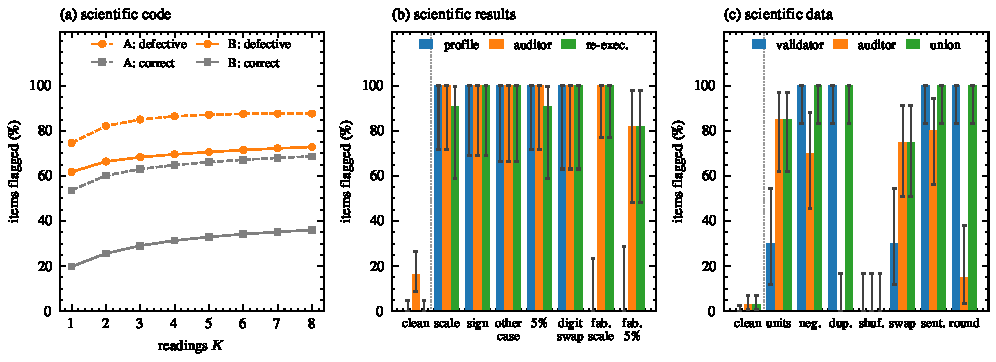
\includegraphics[width=\textwidth]{fig4_ai4s}
  \caption{What each tier flags. (a) Scientific code: the shipped auditor's union flag rate against
  the number of readings, on defective (orange) and correct (grey) instances, in the registered arm
  that gave the whole problem as the task (dashed) and the arm that named the step as the deliverable
  (solid). (b) Scientific results and (c) scientific data, by fault type, with clean items leftmost:
  the deterministic tier (blue: the \texttt{science} profile in b, the card-derived validator in c),
  the LLM auditor at four readings (orange), and re-execution (b) or the union of the two (c) in
  green. Bars carry exact binomial 95\% intervals on the item counts (supplementary; they ignore
  clustering). Registered flag rule throughout: any model BLOCKER in the union of readings.}
  \label{fig:ai4s}
\end{figure*}

\subsection{Scientific code}
\label{sec:ai4s-code}

\textbf{Design.} SciCode \citep{tian2024scicode} decomposes research problems from 16 subfields into
steps with numeric tests written by scientists. The same frozen generator wrote every step three
times, each sample building on its own earlier steps. An instance is correct if it passes the step's
tests and defective if not; a step enters only if some sample passes it. This gives 81 defective
instances (30 problems) and 150 correct ones (53 problems). SciCode has no visible/hidden split, so
the auditor sees the step's prose, background, header and code, and no tests. The shipped
cross-vendor auditor and the generator's own model each read every instance eight times. After the
registered arm's outcomes, a second registered arm changed only the task text, naming the step's
function as the deliverable instead of opening with the whole problem; the program bytes are
identical (Appendix~\ref{sec:ai4s-code-full}).

\textbf{Results.} In these runs, what the auditor was told the deliverable is changed its flag rate
substantially (Figure~\ref{fig:ai4s}a). With the whole problem as the task, the shipped auditor
flagged 87.7\% [72.7, 98.6] of defective and 68.7\% [56.6, 79.7] of correct instances at eight
readings, many of its objections to correct code being that one step did not implement the whole
problem. With the step as the deliverable, flags on correct code fell to 36.0\% [26.4, 45.6], a
paired change of $-32.7$ points [$-42.8$, $-22.4$], and recall fell to 72.8\% [59.3, 87.3], $-14.8$
points [$-28.6$, $-2.7$]. The generator's own model flagged 46.9 points less of the defective
instances than the shipped auditor in each arm (a route comparison). At one reading the shipped
auditor flags 61.7\% of defective against 19.8\% of correct instances: it discriminates, modestly.
A read sample of its flags on correct code ranges from real divergences between code and step text
to contradictions inside the benchmark's own instructions and tests too weak to separate outputs.
Few defects escaped all sixteen readings (7 and 19 in the two arms); most were rated
consensus-undetermined by the prose, but the registered test that this share exceeds the
general-code residual's 77.2\% is killed in both arms by its own interval rule.

\subsection{Scientific results}
\label{sec:ai4s-results}

\textbf{Design.} Each of 74 correct SciCode instances (36 problems) whose output on one seeded test
case is a real scalar or a short real array becomes a results increment: the program, the test's
inputs, a script that runs one on the other and writes a run log, a \texttt{results.json} citing each
value's log line, and a report whose numbers carry the product's number$\to$source annotations. Each
yields a clean item and a faulty one. Five fault types are \emph{reporting} faults, where the
artefacts disagree with each other or with the log; two are \emph{fabrications}, a $\times10^3$ slip
or a 5\% error written consistently into log, results and report. The LLM auditor reads each item
four times with the shipped \texttt{science} profile on, the profile's own verdict comes from the
same call, and re-execution compares the output with the report (Appendix~\ref{sec:ai4s-results-full}).

\textbf{Results.} The deterministic profile flags all 49 reporting faults and none of the 25
fabrications, because in those everything agrees with everything else (Figure~\ref{fig:ai4s}b). The
LLM auditor flags 23 of the 25 fabrications, 21 with a sound finding about the fault (post hoc),
usually by working the result out from the code, for example evaluating a KL divergence to 1 where
the report says 1000; the other two rest on wrong calculations. All 23 discordant items go the LLM's
way (exact McNemar $p = 2.4\times10^{-7}$). On reporting faults its rate is of the combined workflow,
since its prompt carried the profile's findings. Re-execution misses four faults on outputs within
\texttt{np.allclose}'s default absolute tolerance of zero. The LLM also flags 12 of 74 clean items:
8 correctly identify defects in our construction (a provenance sentence false where the benchmark
passes inputs as call literals; a unit label contradicting documented units), 4 rest on wrong
calculations or a syntax error that is not there.

\subsection{Scientific data}
\label{sec:ai4s-data}

\textbf{Design.} Four CC BY 4.0 physical-science tables \citep{yeh1998concrete, brooks1989airfoil,
tufekci2014ccpp, hamidieh2018superconductor}; 280 items of 120 rows with a data card giving each
column's meaning and unit: 140 clean, and 140 carrying one of seven faults (mixed units, negated
values, duplicated rows, a shuffled target, swapped columns, a $-999$ sentinel, rounding). Both model
families read each item four times, against a validator written from the card and frozen before any
item existed (Appendix~\ref{sec:ai4s-data-full}).

\textbf{Results.} The two tiers catch different faults (Figure~\ref{fig:ai4s}c). The validator flags
92 of 140 faulty items (65.7\% [57.9, 73.6]) and no clean item; the shipped auditor 65 of 140 (46.4\%
[38.6, 54.3]) at 4 of 140 clean items (2.9\%); their union 112 (80.0\% [73.6, 86.4]) at the same 4.
Of the 20 faulty items the auditor flags and the validator misses, 18 carry a finding about the
injected fault itself (post hoc), mixed units or swapped columns; in one it argued that three atoms
spanning a 135\,pm radius range cannot have a mean radius of 1.6\,pm, which is the converted cell.
It flagged no shuffled target and no duplicated rows (0 of 20 each), and did worse than the
validator on every fault the validator was written for. The generator's own model flags 67 of 140
clean items, and for at least 48 of those one finding states a row count, field count, missing
column or truncation the file contradicts. The validator omits one range the concrete documentation
states and uses a list of continuous columns the card does not give.
